
\documentclass[colorinlistoftodos]{article} % For LaTeX2e
\usepackage{iclr2020_conference,times}

% Optional math commands from https://github.com/goodfeli/dlbook_notation.
\input{math_commands.tex}

\usepackage{hyperref}
\usepackage{url}
\usepackage[algo2e,ruled,linesnumbered,lined]{algorithm2e}

\usepackage[english]{babel}
\usepackage[utf8]{inputenc}
\usepackage{algorithm}
% \usepackage{arevmath}     % For math symbols
\usepackage[noend]{algpseudocode}


\newcommand\mynotesEB[1]{\textcolor{red}{#1}}
\setlength{\marginparwidth}{3cm}
\usepackage{amssymb,todonotes}


\title{Online Learned Continual Compression via Stacked Quantization Modules}

% Authors must not appear in the submitted version. They should be hidden
% as long as the \iclrfinalcopy macro remains commented out below.
% Non-anonymous submissions will be rejected without review.

\author{Antiquus S.~Hippocampus, Natalia Cerebro \& Amelie P. Amygdale \thanks{ Use footnote for providing further information
about author (webpage, alternative address)---\emph{not} for acknowledging
funding agencies.  Funding acknowledgements go at the end of the paper.} \\
Department of Computer Science\\
Cranberry-Lemon University\\
Pittsburgh, PA 15213, USA \\
\texttt{\{hippo,brain,jen\}@cs.cranberry-lemon.edu} \\
\And
Ji Q. Ren \& Yevgeny LeNet \\
Department of Computational Neuroscience \\
University of the Witwatersrand \\
Joburg, South Africa \\
\texttt{\{robot,net\}@wits.ac.za} \\
\AND
Coauthor \\
Affiliation \\
Address \\
\texttt{email}
}

% The \author macro works with any number of authors. There are two commands
% used to separate the names and addresses of multiple authors: \And and \AND.
%
% Using \And between authors leaves it to \LaTeX{} to determine where to break
% the lines. Using \AND forces a linebreak at that point. So, if \LaTeX{}
% puts 3 of 4 authors names on the first line, and the last on the second
% line, try using \AND instead of \And before the third author name.

\newcommand{\fix}{\marginpar{FIX}}
\newcommand{\new}{\marginpar{NEW}}

%\iclrfinalcopy % Uncomment for camera-ready version, but NOT for submission.
\begin{document}


\maketitle

\begin{abstract}
We \mynotesEB{introduce} and study the problem of Online Continual Compression, where an agent learns to compress a non i.i.d data stream. We propose a new architecture which stacks Quantization Modules (SQM), consisting of a discrete autoencoder equipped with a tiny episodic memory. Every added module is trained to reconstruct the latent space of the previous module using fewer bits, allowing the learned representation to become more compact as training progresses. This modularity has several advantages: 1) moderate compressions are quickly available early in training, which is crucial for remembering the early tasks, 2) as more data needs to be stored, earlier data becomes more compressed, freeing memory, 3) unlike previous methods, our approach \textit{does not require pretraining}, even on challenging datasets. We show two potential applications of this method. We first replace the episodic memory used in Experience Replay with SQM, leading to significant gains on standard CL benchmarks using a fixed memory budget. We then apply our method to LiDAR data, and show results on some downstream task.

\end{abstract}

% \listoftodos
% ---------------------------------------------------------
%                       INTRODUCTION
% ---------------------------------------------------------

\section{Introduction}

\subsection{Motivation for Online Continual Compression}
%Intro paragraph about learned compression
Interest in machine learning in recent years have been fueled by the plethora of data being generated on a regular basis \cite{}. Effectively storing and using this data is critical for their application. Compression can greatly reduce the storage burden in many cases and in others can reduce the memory and compute usage in downstream machine learning applications \citep{JPEG,Oyallon_2018_ECCV}. Thus learned compression has become a topic of interest \cite{VQVAE,ACN,OneMore}. On the other hand its application in reducing the size of datasets bound for machine learning applications has been limited.

%Continual online compression has some natural use cases  
A relatively common situation we highlight is new training data arrives continuously for the learning algorithm to exploit, however this data might not be iid and furthermore it may not be possible to store all the data uncompressed. For example a robotic agent collecting training data might be changing its environment overtime. Similarly autonomous vehicles may collect more diverse data overtime with different objects observed in different environments. A standard learned compression algorithm \cite{torfason2018towards} being continuously learned and adapted on the incoming data is not well designed to deal with this case.  

%Similarly in continual learning for classification replay is important and why not learn to compress
In the field of continual/lifelong learning, which has for now largely focused on classification, approaches based on replay have emerged as some of the most effective. These either store small subsets of the data for later rehearsal or attempt to learn generative models of the data to permit replaying samples of previously seen data distribution\cite{MIR,ER, GenReplay}. Indeed many continual learning application would be solved with replay approaches if you could afford to store all samples. These approaches are thus inherently limited by the amount of data that can be stored in a bounded memory. On the other hand if one attempts to learn to effectively compress samples, the learned compression may itself experience forgetting. Thus a learned compression method that can learn continously would allow the storing of far larger amount of samples for replay.

In this work we rely on quantized autoencoders, specifically the VQ-VAE framework \cite{VQVAE}, observing these can learn continously and online with minimal forgetting, particularly when augmented with their own internal rehearsal mechanisms. For image data we show these can be used to build a multiscale pipeline that allows the compressor to adaptively store samples at different compression scales, based on its effectiveness in compressing that sample.    

Furthermore, learned compression can allow multiple continual learning models to be learned off the same data. 
\todo[color=green]{add motivation related to huge amount of data to compress problem}
To summarize our contributions in this work are as follows:
\begin{itemize}
    \item We introduce and highlight the importance of the online continual learned compression problem
    \item We demonstrate how Multi-level VQ-VAE combined with rehearsal\cite{MIR,ER} can be effective at this problem
    \item We show state-of-the-art performance in X,Y,Z
\end{itemize}


\begin{enumerate}
	%\item Learned Compression (in general)
	%\begin{enumerate}
	%	\item  Amount of data being generated on a regular basis is huge (cite article Mass was referencing). 
	%	\item Reduce storage burden, Make the most of your storage capacity (especially for high-performance / low memory hardware like GPU)
	%\end{enumerate}

	%\item Online Compression
	%			\begin{enumerate}
	%				\item There might not always be pretrained models available for all data types (think of LiDAR for example). The need sample efficient convergence / performance can be crucial, especially for applications where collecting data is expensive (more in the robotics section)
	%			
	%			\end{enumerate}						

	
%	\item Robotics Perspective 
%		\begin{enumerate}
%			\item  Deploying robots for high-dimensional data collection in the wild. 
		
%			\begin{enumerate}
%				\item Scenario A: Robot is collecting data without access to internet, and with limited storage capacity. There is an overhead cost for it to come back to a docking station and transmit its data. E.g a rover on the moon. 
%				\item Scenario B: Robot must transmit data over bandwidth. Less bits transmitted $\rightarrow$ Cost of transmission is reduces		
%			\end{enumerate}	
			
%			\item Expensive to operate robots (I would assume Le Bras Canadien in space is one of them). If you are going to train an AI to perform some complex manipulation task, you will want to train it with a few samples as possible. (This is more to motivate the \textit{online} part.	 
		
%		\end{enumerate}				
			
		%\item Continual Learning
		%	\begin{enumerate}
			%	\item Storing data (and compressed versions of it) is much more robust to forgetting (than regular approaches); \textbf{the data holds all the information you need to train a model}. The problem is that memory quickly becomes the main hurdle to overcome. By compressing the data you can alleviate this obstacle. 
			%	\item Small Note: I would like to stress the point above, that most online CL application would be solved with memory-based approaches if you could afford to store all samples.
			%	\item SOTA methods for CL are largely rehearsal based.  Same argument as below: storing compressed representations not only allows you to store more, but makes rehearsal more efficient
		%	\end{enumerate}
			
				
		\item Deep Learning Perspective
			\begin{enumerate}
				\item Memory NNs / Nonparametric Approaches
				\begin{enumerate}
					\item GPU memory is small and limited. A major bottleneck in training models is the RAM to GPU transfer. If you are dealing with compressed representations the transfer time per example is smaller, hence makes training faster. 
					\item This would be especially true for networks that leverage an external memory during training / inference (hence the title). 
				\end{enumerate}		

			\end{enumerate}
 
\end{enumerate}

\todo[color=green]{finish introduction}


% ---------------------------------------------------------
%                       RELATED WORK
% ---------------------------------------------------------
\section{Related Work}

Closely related to our work \cite{scalable2017} consider compressing memories for use in the continual classification task. They also employ a discrete latent variable model but with the Gumbel approximation which shows to be far effective than our approach based on \cite{VQVAE}. 
\begin{enumerate}
    \item Continual Learning / CL for Robotics
    \item Quantization and Compression
    \item DGM Lidar \citep{caccia2018deep}
    \item Online Learning ?
\end{enumerate}

\todo[color=green]{finish related works}

% ---------------------------------------------------------
%                      Motivation & Understanding
% ---------------------------------------------------------

\section{Motivation / Why this works}
\begin{enumerate}
    \item Deep Generative Modeling, unlike discriminative tasks, is much harder to overfit. This allows us to do multiple iterations over the same minibatch, hence more sample efficient learning. 
    \item VQ-VAEs learn surprisingly fast; something about learning a codebook, and having a deterministic encoding.
    \item On that note, training modules independently leads to faster convergence. Could we show something about the variance of the gradients ? (if you train whole thing together, more params, so variance add up)
    \item Distillation
\end{enumerate}


% ---------------------------------------------------------
%                      Approach
% ---------------------------------------------------------

\todo[color=red]{sketch out the entire Methodology section}

\todo[color=yellow]{finish Methodology section}

\section{Methodology}
In this section we outline our approach to the online continual compression problem. Our learned compression network consists of a set of Multi-resolution VQ-VAE blocks. These blocks only communicate information forward and are not learned jointly unlike the \cite{VQVAE-multi}. Memories are compressed using an adaptive scheme that controls what resolution the sample is stored, and therefore how compressed the sample should be. Furthermore memories can be revisted and further compressed as the learned compression module improves. Finally a rehearsal phase that utilizes the stored memory is used to minimize forgetting and update representations stored in the memory. 

\subsection{Vector Quantized VAE}
Variational Autoencoders (VAE) consist of two parts: the encoder network parameterizes the posterior distribution $q(z|x)$ and the decoder network $p(x|z)$ aims to reconstruct the original input $x$ from the inferred latent variables $z$. Both the prior and posterior distributions are usually Gaussian with diagonal covariance. 

Vector Quantized Autoencoders (VQ-VAE) use a discrete latent representation instead. This model additionally keeps an embedding table $E \in \mathbb{R}^{K \times D}$, consisting of $K$ vectors of size $D$. Given an RGB image, the encoder first encodes it as a $H_h \times W_h \times D$ tensor, where $H_h$ and $W_h$ denote the height and width of the latent representation. Then, every $D$ dimensional vector goes through a discretization bottleneck using a nearest-neighbor lookup on the embedding table. Specifically, 

\begin{equation*}
    z_{ij} = \argmin_{e \in E} || \texttt{enc}(x)_{ij} - e ||_2
\end{equation*} 

The output of the discretization step is then fed through the decoder to recover an RGB image. The gradient of this  non-differentiable step is approximated using the straight-throught estimator. A key property to notice is that to reconstruct the input, only the $H_h \times W_h$ indices are required, since the embedding table is shared across samples. This property lies at the heart of our approach. 

\subsection{Stacked Quantization Modules}
\begin{figure}
    \centering
    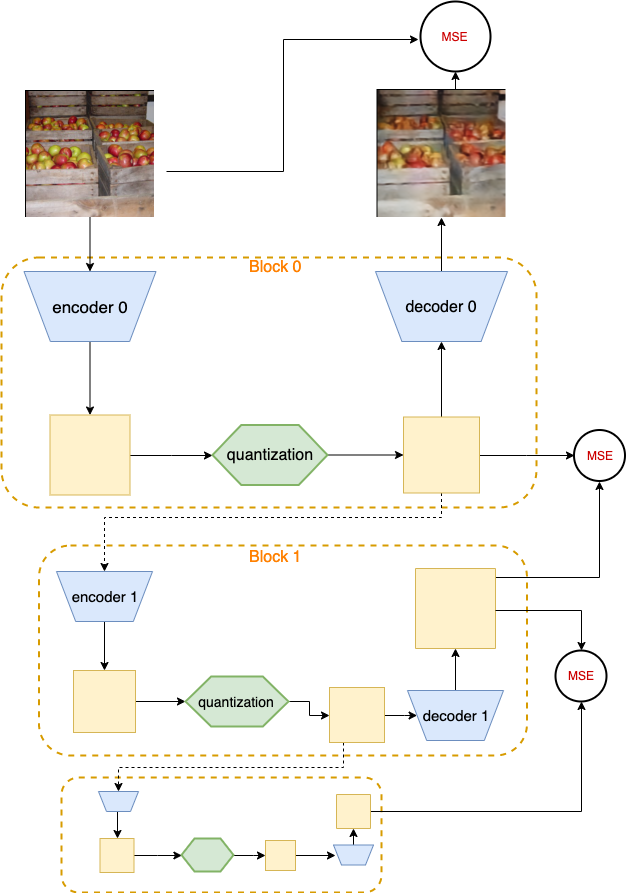
\includegraphics[width=0.6\linewidth]{figs/sqm_cartoon.png}
    \caption{dotted lines means the gradient is stopped in the backprop}
    \label{fig:soft_modules}
\end{figure}

We now describe the proposed XXXXX . Each module contains a VQ-AE and a corresponding index buffer of adaptive capacity. Its input is the $z_q^{(i-1)}$ from the previous layer. Unlike \cite{}, each module is learned greedily without backward communication between modules. This formulation is important for allowing the moudles to each converge as quickly as possible at their respective resolution, important for online continual learning.  A full diagram of the XXXX is given in Figure~\ref{fig:soft_modules}

Each module reconstructs its input from latent representation $z_q^{i}$, where $\textsc{BITS}(z_q^{i}) < \textsc{BITS}(z_q^{(i-1)})$. The compression rate is given by
    $$
        \frac{H \times W \times C \times  \log_2{(256)}}
             {N_c \times H_h_i \times W_h_i \times \log_2{(K_i)}}
    $$
    Thus the compression rate is controlled by 3 variables : $K_i$, the number of embeddings in the codebooks of block $i$, The spatial dimension of the latent rep ($H_{hi}$, $W_{hi}$) and the number of codebooks $N_c_i$ 
%\begin{enumerate}
    %\item Its input is the $\textsc{STOP GRADIENT}(z_q^{(i-1)})$ from the previous layer. 
%    \item Module reconstructs its input from latent representation $z_q^{i}$, where $\textsc{BITS}(z_q^{i}) < \textsc{BITS}(z_q^{(i-1)})$
 %   \item The compression rate is given by
 %   $$
  %      \frac{H \times W \times C \times  \log_2{(256)}}
   %          {N_c \times H_h_i \times W_h_i \times \log_2{K_i)}}
    %$$
    %Meaning you have three knobs to turn to abjust the compression rate: $K_i$, the number of embeddings in the codebooks of block $i$, The spatial dimension of the latent rep ($H_{hi}$, $W_{hi}$) and the number of codebooks $N_c_i$ 
%\end{enumerate}


\subsection{Modular Training}
\begin{enumerate}
    \item Allows for faster convergence, as the bottom most block is not required to build representations which account for all levels of compression. Faster convergence translates to more knowledge being retained, as the effective capacity of the network quickly grows (b/c you can store good compressions)
    \item Minimizes interference. Each block receives local updates. Something along the lines that variance of the updates should be smaller as you are adding fewer random variables. Maybe make some bs link with the biologically plausible backprop, which requires "local" learning updates
    \item TODO: would allow fully in parallel and asynchronous training, could even rehearse on different points (link to MIR)
    
    \item TODO: (maybe put this somewhere else). Regular VQ-VAEs usually use exponential moving averages to update the codebook. However we found this optimization, while being more performant in reconstruction error, to be more vulnerable to drifting representations. (See ablation study)

    
    
\end{enumerate}

\subsection{Multi-Level Storage}
The Hierarchical part  serves two purposes
\begin{enumerate}
    \item Allow knowledge retention before the compressor networks learning valid representations. This is crucial for tasks with few datapoints; If compressor has not yet converged, storing poor latent reps. will result in this task being fully forgotten
    \item Compression difficulty not the same for all datapoints. This allows to use more capacity for harder data and, fewer for more simple points.
\end{enumerate}

\subsection{Multi-Level Reservoir Sampling}
Reservoir Sampling (RS) is the workhorse of rehearsal based methods. Its popularity is due to two reasons. First, it gives in expectation a sample representative of the whole data stream.  Second, it is conceptually simple algorithm, easy to implement, and gives strong empirical results. \\
Mention that more sophisticated approached (such as ER-Ringbuffer ER-Kmeans in \url{https://arxiv.org/pdf/1902.10486.pdf} are outperformed by simpler RS) \\

With this motivation, we wish to adapt RS to a multi-level settings. There a a few challenges 
\begin{enumerate}
    \item \textbf{Capacity is not fixed.} RS adds a new point with prob. $p=\frac{\text{buffer capacity}}{\text{points seen so far}}$. However in practice the buffer capacity increases as the compressor network gets better. We therefore estimate it using the current capacity at the time of buffer addition
    \item On the same argument, one could argue that in practice the compressor network's capacity is actually bigger than the amount of samples it's currently storing since old samples were added when the buffer was less performant. However, since the points get recompressed during rehearsal, this issue is mostly addressed.
    \item \textbf{Sample Selection} for deletion and sampling. While it would be more advantageous to remove datapoints from the least compression representations, doing so introduces a bias; some classes may be harder to compress, and remove them favorably would result in more forgetting of said class. We therefore select points to be deleted in a fully compression agnostic way.
    
\end{enumerate}


%           ALGORITHMS 
% ---------------------------------------------------------


%               TRAINING LOOP 
% ---------------------------------------------------------
\begin{minipage}{0.99\textwidth}
\begin{algorithm2e}[H]\small
\SetAlgoLined
  \DontPrintSemicolon
    \KwIn{Learning rates $\alpha_{cls}$, $\alpha_{ae}$ }
 \textbf{Initialize:} Memory $\mathcal{M}$; $\theta_{cls}$, $\theta_{ae}$ \\
\For{$t \in 1..T$}{

    \,\,\,\texttt{\% Fetch data from current task}\\
    \For{$B_{inc}\sim D_t$}{
    
        \,\,\,\texttt{\% Perform multiple passes over the incoming batch}\\
        \For{$n \in 1..N$}{
            $B \gets B_{inc}$ \\
            \If{$t > 1$}{
            
                \,\,\,\texttt{\% Fetch data from previous tasks}\\
                $B_{re}$ \sim \textsc{Sample}({M})\\
                $B$ \gets (($B_{inc}$, $B_{re}$)) \\
            }
            
            \,\,\,\texttt{\% Train Compressor Network}\\
            \theta_{gen} \gets ADAM(B, \alpha_{ae})$ \\
            
            \,\,
            \If{$ t > 1$}{
                \textsc{Update Buffer}(M, \theta_{ae}) \\
            }

        \,\,\,\texttt{\%Save current latent indices}\\
        \textsc{ADD TO MEMORY}({M}, $B_{inc}$, \theta_{ae})\\
        
        }
    }
}

\caption{ Multi-Level Vector Quantized Replay}
\label{algo:vqr}
   % \end{edit}
\end{algorithm2e}
\end{minipage}


%           Find Most Compact Representation 
% ------------------------------------------------------
\begin{minipage}{0.99\textwidth}
\begin{algorithm2e}[H]\small
\SetAlgoLined
  \DontPrintSemicolon
    \KwIn{datapoint $x$, Autoencoder $AE$ with $L$ levels, distortion threshold $d_{th}$}
 \textbf{Initialize:} Memory $\mathcal{M}$; $\theta_{cls}$, $\theta_{ae}$ \\
 
 \,\,\,\texttt{\% Do a full encoding pass to compute hidden rep. for all blocks} \\
 \textst{ENCODE}($AE$, $x$)
 
\,\,\,\texttt{\% Iterate over blocks, from most compressed to less compressed}\\
\For{$i \in T..1$}{

    \,\,\,\texttt{\% Fetch latent indices and hidden rep. computed in forward pass}\\
    argmin$_i$, $z_q$ = \textst{ARGMIN}($block_i$)
    
    \,\,\,\texttt{\% Decode to output space} \\
    \For {$j \in i...1$}{
        \,\,
        $z_q$ = \textst{DECODE}($block_j$, $z_q$)
    }
    
    \,\,\,\texttt{\% Compute distortion between both images} \\
    err = \textst{MSE}($\tilde{x}$, $z_q$)
    
    \,\,
    \If{$err < d_{th}$}{
        \textbf{return} argmin$_i$, \ $i$
    }
}

\,\,\,\texttt{\% If no compression is good enough, return original image} \\
\textbf{return} $x$, 0


 
 \caption{\textst{AdapCompress}: Find Compact Representation}
\label{algo:vqr}
   % \end{edit}
\end{algorithm2e}
\end{minipage}


%           BUFFER INDEX UPDATE
% ---------------------------------------------------------
\begin{minipage}{\textwidth}
\begin{minipage}{0.45\textwidth}
\begin{algorithm2e}[H]\small
\SetAlgoLined
  \DontPrintSemicolon
    \KwIn{Memory $\mathcal{M}$, Autoencoder $AE$ with $L$ levels, data $D$, distortion threshold $d_{th}$}
    
\For{$x \in D$}{
    $hid_x$, $block_{id}$ = \textst{AdapCompress}($x$, $AE$, $d_{th}$) \\
    
    \,\,\,\texttt{\% Delete Old Repr.} \\
    \textst{DELETE}($\mathcal{M}$[$x$]) \\
    \,\,\,\texttt{\% Add new one} \\
    \textst{ADD}($\mathcal{M}$, $hid_x$) 
}

 \caption{Update Buffer Representations}
\label{algo:vqr}
    
   % \end{edit}
\end{algorithm2e}
\end{minipage}
\qquad
%           RESERVOIR ADD 
% ------------------------------------------------------
\begin{minipage}{0.5\textwidth}
\begin{algorithm2e}[H]\small
\SetAlgoLined
  \DontPrintSemicolon
    \KwIn{Memory $\mathcal{M}$ with capacity $C$, sample $x$}
    
    \,\,\,\texttt{\% Calculate number of uncompressed samples buffer can store} \\
    $N_{reg}$ = $\frac{C}{\textst{BYTES}(x)}$
    
    \,\,\,\texttt{\% Calculate probability of adding incoming datapoint} \\
    
    capacity = $\max$(\ $N_{reg}$, \textst{CURRENT SAMPLE AMT}($\mathcal{M}$)\ ) 
    
    \,\,\,\texttt{\% Calculate probability of adding incoming datapoint} \\
    add $\sim \mathcal{B}(\frac{\text{capacity}}{\text{SAMPLE AMT SEEN SO FAR}})$
    
    \,\,
    \If{add}
    {
        $hid_x$, $block_{id}$ = \textst{Find Compact Representation}($x$, $AE$, $d_{th}$) \\
        space missing =  \text{BYTES}($hid_x$) - \textst{FREE SPACE}($\mathcal{M}$)
        
        \,\,\,\texttt{\% Note: implementation is much faster but same idea} \\
        \While {\text{space missing}}{
            \textst{DELETE RANDOM POINT}($\mathcal{M}$) \\
            space missing =  \text{BYTES}($hid_x$) - \textst{FREE SPACE}($\mathcal{M}$)
        }
        
    }
    

 
 \caption{Add to Memory}
\label{algo:vqr}
   % \end{edit}
\end{algorithm2e}
\end{minipage}
\end{minipage}

%          End of Algorithms Section 
% ------------------------------------------------------


\subsection{Architectural}
\begin{itemize}
    \item Define a VQVAE block
    \item Describe the Modular Stacking 
    \item Tensor Quantization ! vs vector
\end{itemize}

\subsection{Representation used for LiDAR}
\begin{itemize}
    \item describe padding for rotational equivariance
\end{itemize}

\subsection{Optimization}
\begin{itemize}
    \item Blockwise vs Full
    \item Distillation
    \item Criterias to spawn a new module
    \item How to init new blocks ?
\end{itemize}



\subsection{Using Index Collapse to our advantage}
\begin{itemize}
    \item Start with a high number of embeddings. 
    \item When replaying, reorder and compress the codebook! Underuse of embeddings is not a bad thing for compression --> less bits per items
\end{itemize}

\subsection{What about resampling unused codebook vectors?}

% ---------------------------------------------------------
%                      Experiments
% ---------------------------------------------------------
\section{Experiments}

We evaluate the efficacy of the proposed methods on a suite of canonical and new experiments. In Section \ref{sec:exp_details}, we describe the experimental setting. Section \ref{sec:can_cl} presents results on standard supervised continual learning benchmarks. We choose datasets on the more challenging side of the evaluation protocols proposed thus far. Moreover, we introduce a new online compression task on less orthodox data, i.e. LiDAR, to demonstrate the generality of our approach.

\subsection{Experimental Setting}
\label{sec:exp_details}


\paragraph{Supervised Continual Learning}


\paragraph{On the test-time task label assumption} Shared head rules, however multi-head (closer to multi-tasking) can be useful in e.g. robotics. We are so nice that we studied both settings.

\paragraph{Baselines}
Our first and foremost baseline for continual supervised learning is Experience Replay (ER). It consists of storing old data in a buffer to replay old memories. Due to its oversimplistic nature, this baseline was omitted in most continual learning papers. However, recent research made it clear that it is a much difficult to beat baseline and in some settings it is state-of-the-art \citep{chaudhry2019continual,aljundi2019online,aljundi2018Online} \todo{cite more?}. This is the most important baseline as our method is an add-on to ER. Thus, the difference in performance will inform us about the efficacy of SQM and A-SQM. Here is a list of the other baselines in the supervised learning experiment:
\begin{itemize}
    \item \textbf{iid online} (upper-bound)
    considers training the model with a single-pass through the data on the same set of samples, but sampled iid.
    \item \textbf{iid offline} (upper-bound)
    evaluates the model using multiple passes through the data, sampled iid. We use 5 epochs in all the experiments for this baseline.
    \item \textbf{fine-tuning} 
    trains continuously upon arrival of new tasks without any forgetting avoidance strategy.
    \item \textbf{iCarl} \cite{rebuffi2017icarl} introduced 
    \item \textbf{GEM} \cite{lopez2017gradient} proposed a rehearsal methods that ... It gives similar results to the recent A-GEM \cite{chaudhry2018efficient}. 
    \item  \textbf{MIR} \cite{aljundi2019online} proposed another rehearsal method that 
\end{itemize}

Our other baselines are compression specific and are used in the supervised continual learning experiment as well as the LiDAR one. 


\begin{itemize}
    \item Continuous AE
    \item Gumbel AE
    \item Argmax AE
\end{itemize}



\subsection{Canonical Evaluations for Supervised Continual Learning}
\label{sec:can_cl}

In this section, we study the proposed methodology under the standard evaluation protocol for CL: incremental image classification. The more challenging datasets which as been studied thus far are CIFAR (cite) and Mini Imagenet. The former as been studied 

\todo[color=red]{insert preliminary results for continual supervised learning}
\todo[color=orange]{Describe continual supervised learning results}
\todo[color=yellow]{insert final results for continual supervised learning}


%%%% CIFAR-10
\begin{table}
    \centering
    \resizebox{\textwidth}{!}{%
    \begin{tabular}{ll}
    \begin{tabular}{c c c}
&\multicolumn{2}{c}{Accuracy} \\\hline
                 & $M=20$ & $M=50$  \\\hline \hline
    iid online     &$60.8\pm1.0$ &$60.8\pm1.0$\\
    iid offline     &$79.2\pm 0.4$ &$79.2\pm 0.4$\\\noalign{\hrule height 1pt}
    GEM   \citep{lopez2017gradient}   &$16.8 \pm 1.1$& $17.1 \pm 1.0$\\
    iCarl (5 iter)  \citep{rebuffi2017icarl}   &$28.6 \pm 1.2$ & $33.7 \pm 1.6$ \\
    fine-tuning &$18.4\pm0.3$& $18.4\pm0.3$\\
     ER&$27.5\pm 1.2$ &$33.1\pm 1.7$\\
    ER-MIR \citep{aljundi2019online}& $29.8\pm1.1$ &$40.0 \pm 1.1$ \\
    SQM (ours) & & $\bm{45.9 \pm 1.1}$\\
    A-SQM (ours) & & $\bm{46.2 \pm 0.6}$ \\
    % \multicolumn{4}{c}{}\\
\end{tabular}
&
\begin{tabular}{c c}
\multicolumn{2}{c}{Forgetting} \\\hline
     $M=20$ & $M=50$  \\\hline \hline
    N/A &N/A\\
   N/A&N/A\\\noalign{\hrule height 1pt}
        $73.5 \pm 1.7$ & $70.7 \pm 4.5$ \\
    $49 \pm2.4$& $40.6\pm1.1$\\
  $85.4 \pm 0.7$  & $85.4 \pm 0.7$\\
    $50.5\pm 2.4$&$35.4\pm 2.0$ \\
    $50.2\pm 2.0$&$30.2 \pm 2.3$ \\
    & $36.5 \pm 1.2$ \\
    & $36.1 \pm 0.6$ \\
       %  \multicolumn{4}{c}{}\\
\end{tabular}
\end{tabular}
}
\caption{Shared head results on disjoint CIFAR-10. Total memory per class $M$ measured in sample memory size. We report  (a) Accuracy, (b) Forgetting (lower is better). }
\label{tab:cifar10_er_main}
\end{table}



\subsection{On convergence speed}
\begin{itemize}
    \item Can we justify the convergence speed by looking at the variance in the gradient ?
    \item Can we show that deeper modules need more rehearsing ? We could look at the speed of drift in the reconstructions. 
\end{itemize}

\subsection{Reusing Encoder modules}
\begin{itemize}
    \item In Image classification for RGB data. See \url{https://arxiv.org/pdf/1803.06131.pdf}
    \item 
\end{itemize}

\subsection{Is ER enough to properly decorrelate temporally adjacents frames ?}

% ---------------------------------------------------------
%                      Ablation Study
% ---------------------------------------------------------

\todo[color=orange]{add preliminary results of quality/diversity space ablation}

\section{Ablation Study}
\begin{itemize}
    \item Show that modular training does not hurt final performance (i.e. same compression ratio with only 1 quantization). This will entail that you get compressed intermediate representations for free. 
    \item Show that modular training converges faster! If you train the same fixed architecture altogether, look at the time it takes for the first block to reach some fixed error rate. 
    \item Full Architecture from the start vs Progressive Training. Does it hurt performance ? To be checked
\end{itemize}

% ---------------------------------------------------------
%                      Conclusion
% ---------------------------------------------------------
\section{Conclusion}
\todo[color=green]{finish conclusion}

\clearpage
% ---------------------------------------------------------
%                      TODOs / Misc
% ---------------------------------------------------------
\section{Remaining stuff}

\begin{enumerate}
    \item Would be nice to have a fully mapping task for LiDAR. Say you deploy a robot in an unknown environment, and you want it to collect data. Given a fixed memory, compression becomes really important!

    \item Classification Task for LiDAR ? SLAM, or 3D object detection from point clouds 
    I would like said task to be super close to real life
    \begin{enumerate}
        \item Data comes in temporally corelated $\rightarrow$ Can ER solve this ?
        \item Semi-Supervised setting: only a few frames have labelled objects. This would make the importance of large buffer more important, as it takes a lot of data to properly decorellate frames (TODO)
                
    \end{enumerate}
    
        
    \item Link with MIR: How much does codebook overlap predict forgettability ?
    
    \item Can we show than when a DGM doing compression (vs DDM) has learned a concept, less rehearsal is needed ? Would motivate latent rehearsal

\end{enumerate}
%\subsubsection*{Author Contributions}
%If you'd like to, you may include  a section for author contributions as is done
%in many journals. This is optional and at the discretion of the authors.

%\subsubsection*{Acknowledgments}
%EB acknowledges funding from IVADO


\bibliography{iclr2020_conference}
\bibliographystyle{iclr2020_conference}

\appendix
\section{Appendix}
You may include other additional sections here. 

\end{document}
